\documentclass[11pt]{article}

%FOR SCRIBES: Please change the next three lines to reflect the correct
%FOR SCRIBES: lecture number, name, and date.
\newcommand{\lecturenumber}{0}
\newcommand{\scribename}{{Mridul Gupta}}
\newcommand{\lecturedate}{29 March 2022} 

\usepackage{subfigure}
\usepackage{color}
\usepackage{url}
\usepackage{graphicx}
\usepackage{fullpage}
\usepackage{mathtools}
\newcommand{\etal}{{\em et al.}}
\newcommand{\qed}{\mbox{}\hspace*{\fill}\nolinebreak\mbox{$\rule{0.6em}{0.6em}$}}
\newcommand{\expect}{{\bf \mbox{\bf E}}}
\newcommand{\prob}{{\bf \mbox{\bf Pr}}}

%--------------------------- Commands and Environments I added -----------------
\usepackage[english]{babel}
\usepackage{amssymb}
\usepackage{amsmath}
\usepackage{fancyhdr}
\renewcommand{\baselinestretch}{1.10}
%%      Fonts:
%%---------------------------------------------------------------------------
\newfont{\bssten}{cmssbx10}
\newfont{\bssnine}{cmssbx10 scaled 900}
\newfont{\bssdoz}{cmssbx10 scaled 1200}

%---------------------------------------------------------------------------
\newcounter{topic} \setcounter{topic}{0}
\newcommand{\topic}[1]{\par \refstepcounter{topic} {\bssdoz \arabic{topic}.~ #1} \par}
%\newcommand{\topic}[1]{\par \refstepcounter{topic} \vs{2ex} {\bssdoz \arabic{topic}.~ #1} \par \vs{1ex}}

%------------------------------ end of new commands and evironments ------------

\definecolor{gray}{rgb}{0.5,0.5,0.5}
\newcommand{\comment}[1]{{\color{gray}[\textsf{#1}]}}
\newcommand{\redospace}{\small\renewcommand{\baselinestretch}{1.5}\normalsize}
\newcommand{\undospace}{\small\renewcommand{\baselinestretch}{1}\normalsize}
\newtheorem{theorem}{Theorem}[section]
\newtheorem{lemma}[theorem]{Lemma}
%----------------------------- some other things I added ---------------------
\newtheorem{claim}[theorem]{Claim}
\newtheorem{example}[theorem]{Example}
\newtheorem{protocol}[theorem]{Protocol}
%----------------------------------------------------------------------------
\newtheorem{corollary}[theorem]{Corollary}
\newtheorem{definition}{Definition}[section]
\newtheorem{remark}[definition]{Remark}
\newtheorem{conjecture}[theorem]{Conjecture}
\newtheorem{proposition}[theorem]{Proposition}
\newenvironment{proof}{{\bf Proof:}}{$\qed$\par}
\newenvironment{proofof}[1]{{\bf Proof of #1:}}{$\qed$\par}
\newenvironment{proofsketch}{{\sc{Proof Outline:}}}{$\qed$\par}

\usepackage{hyperref}
\hypersetup{
	bookmarksnumbered
}


	
	\begin{document}
		%{	\color{blue}   \textbf{Edit the parts in blue and remove this part}}
		\begin{center}
			\framebox{\parbox{6.5in}{
					{\bf{ELL888 Indian Institute of Technology Delhi} }\\ 
					{\bf  {\color{blue} {MCM Kernel Optimization}}}
					\\
{Scribed by: {\color{blue}\textit{Mridul Gupta (2021AIZ8322)}}\\ Instructors:
						 Sandeep Kumar and Jayadeva}
			}}
			\ \\
		\end{center}
%		\noindent{\bf Note}: {LaTeX template courtesy of UC Berkeley EECS dept.}
		
		\noindent {\bf Disclaimer}: {These notes have not been subjected to the
			usual scrutiny reserved for formal publications.  They may be distributed
			outside this class only with the permission of the Course Coordinator.}
		\vspace*{4mm}
		\setcounter{section}{\lecturenumber}
		%FOR SCRIBES: ---------- Begin Scribing Here ------------------------
	
\tableofcontents
\section{Structure}
Structure these points later
    \begin{itemize}
        \item[$\boxtimes$] Class separability might be worse in the feature space.
        \item Start with we want to get a bound on the risk on the test data. This
            requires knowing the distribution from which the data is being generated.
        \item We cannot know the distribution parameters. So, we estimate the actual risk
            using empirical risk which is the risk given some (training) samples from the
            distribution.
        \item Risk bound equation in VC slt.pdf
        \item Highlight two parts, the empirical risk and the structural risk
        \item make note that to reduce risk, we must reduce h (VC-Dimension)
        \item Mention VC-Dimension bound for $\Delta$-margin classifiers.
        \item Mention that in general it will be $n+1$ but it can be bound by reducing
            $\displaystyle \dfrac{R^2}{\Delta^2}$
        \item Show the simplified graph
        \item This transformation might not take to same dimensional space, might be
            higher dimensional. This function is a Kernel, that needs to be optimized to
            optimize structural risk.
        \item Also mention examples why sometimes even an infinite dimensional kernel
            might not work. And why we need Kernel Optimization.
        \item Go into the details of how to do this.
        \item Mention appropriate theorems, definitions and lemmas in between.
        \item Add a key takeaways section.
    \end{itemize}

Refined list to structure
    \begin{itemize}
        \item A little intro to MCM (slt, minimize vc dim bound, structural risk minimization).
        \item What is kernel optimization, why it is needed
        \item Amari's idea, magnifying around support vectors
        \item Xiong's idea of using a scatter matrix, Fisher discriminant
        \item Xiong's idea of creating a kernel scatter matrix, how it's equal to normal scatter
        \item Empirical feature space, matrix equations
        \item solving generalized eigenvalue problems
        \item Getting the MCM with optimized kernel
    \end{itemize}


\section{Introduction}
Support Vector Machines (SVMs) are older than the state of Haryana (the linear variant at
least), and the kernel version of SVMs were proposed by Vapnik \etal\ in 1992. Vapnik and
Chernvonenkis along with others also developed theory key thoeretical concepts that
constitute statistical learning theory. In what follows, we will discuss the theoretical
and practical advancements since then that led to the work titled ``Kernel optimization
using conformal maps for the minimal complexity machine'' by Jayadeva \etal\par
Since this is the congruence of two paths, one leading to MCMs and the other leading to
kernel optimization in a data dependent way, in the following we first discuss MCMs, and
then kernel optimization, and finally how the two fit together.


\section{Background}
The key concepts that lead to MCMs were available in statistical learning theory long ago,
but weren't applied until 2015. So let's discuss the key concepts that naturally lead to
minimal complexity machines.

\subsection{Statistical Learning Theory}
It all starts by stating the objective of Machine Learning. The model of
learning from examples can be descibed using three components~\cite{slt}:
\begin{enumerate}
    \item a generator of random vectors $x$, drawn independently from a fixed
        but unknown distribution $P(x)$;
    \item a supervisor that returns an output vector $y$ for every input vector
        $x$, according to a conditional distribution function $P(y\;\lvert\;x)$,
        also fixed but unknown;
    \item a learning machine capable of implementing a set of functions
        $f(x,\alpha), \alpha\in\Lambda$.
\end{enumerate}
The problem of learning then is to choose the ``right'' function from the family
of functions $f(x,\alpha), \alpha\in\Lambda$. We want to choose this function so
that it predicts the supervisor's response on seen as well as previously unseen
data in the best possible way. The function choice has to be made based on a set
of pairs $\{(x_i,y_i)\}_{i=1}^M$ called the training set. These samples are
drawn from the distribution $P(x)P(y\;\lvert\;x)$ which is the joint
distribution $P(x,y)$. The $M$ samples are assumed to be {\em independent and
identically distributed (i.i.d.)}.\par
Next we need to define what ``predicting the response in the best possible way
means''. For this we need to define how correct is $f(x,\alpha)$ is compared to
$y$. This is done by defining an error function (also called loss function or
cost function) that assigns some real valued number to two objects (may be
vectors, matrices, scalars, or general mathematical objects). This number
represents the ``cost`` incurred by predicting $f(x,\alpha)$ given $y$.\par
The next important quantity is the {\em risk functional} which is the
expectation of loss. Since, $x$ is a random vector, so the output of
$f(\cdot,\alpha)$ is also random, so is the loss $\mathcal{L}$. Thus, it makes
sense to take the expectation of it.
\begin{equation}
    R(\alpha)=\mathbb{E}_{(x,y)\sim
    P(x,y)}\biggl[\mathcal{L}\bigl(y,f(x,\alpha)\bigr)\biggr]=\int
    \mathcal{L}\bigl(y,f(x,\alpha)\bigr)dP(x,y)
\end{equation}
The goal is then to find $\alpha^*$ that minimizes the risk functional
$R(\alpha)$. The problem is that $P(x,y)$ is unknown, all that's known is the
training set $\{(x_i,y_i)\}_{i=1}^M$.\par
What we do have then is:
\begin{equation}
    R_{\text{emp}}(\alpha)=\frac{1}{M}\sum_{i=1}^M
    \mathcal{L}\bigl(y,f(x,\alpha)\bigr)
\end{equation}
$R_{\text{emp}}$ is called the {\em empirical risk}. Given these quantities, we
have the following result from statistical learning theory:
{\theorem (Vapnik) If $0\le\mathcal{L}\bigl(y,f(x,\alpha)\bigr)\le
B,\alpha\in\Lambda$, that is the loss is totally bounded, then with
probability at least $1-\eta$ the inequality
\begin{equation}
    \label{eqn:pac}
    R(\alpha)\le
    R_{\text{emp}}(\alpha)+\frac{B\varepsilon}{2}\Biggl(1+\sqrt{1+\frac{4R_{\text{emp}(\alpha)}}{B\varepsilon}}\Biggr)
\end{equation}
holds true simultaneously for all functions of the set
$\mathcal{L}\bigl(y,f(x,\alpha)\bigr)$. where
\begin{equation}
    \varepsilon = 4\frac{h\biggl(\ln\frac{2M}{h}+1\biggr)-\ln\eta}{M}
\end{equation} and $h$ is the VC-dimension of the set of functions.}\par
On the RHS of equation~\ref{eqn:pac}, the term other than the empirical risk
$R_{\text{emp}}(\alpha)$ is called the {\em structural risk}.\par
Another important result from Vapnik that will be needed to continue our
discussion of MCMs is:
{\theorem (Vapnik) Let vectors $x\in X$ belong to a sphere of radius $R$. Then
the set of $\Delta$-margin separating hyperplanes has the VC-dimension $h$
bounded by the inequality
\begin{equation}
    \label{eqn:vcbound}
    h\le\min\left(\left[\frac{R}{\Delta}\right]^2,n\right)+1.
\end{equation}} where $n$ is the feature dimension of the data.
For more, refer~\cite{slt}, but for our discussion this is sufficient.\par
\subsection{Minimal Complexity Machines}
\subsubsection{Motivation}
We want to minimize the actual {\bf risk}, $R(\alpha)$, in order to generalize
prediction on future samples. We can do this by tightening the bound on the RHS
of equation~\ref{eqn:pac}. We can optimize the empirical risk, and we can
optimize the structural risk. Note that in structural risk, the only thing we
can alter is $\varepsilon$. We need to minimize $\varepsilon$ to tighten the
bound on the risk. And in the expansion of $\varepsilon$ we can only alter $h$
assuming the training sample size is as large as we can get.
$\varepsilon\propto h$. Thus to reduce $\varepsilon$, we want to minimize
$h$.\par
Now let's look at figure~\ref{fig:1}. Imagine we have the data points in
$\mathbb{R}^1$. The blue dot shows the optimal hyperplane that classifies the
points with maximum margin. $R$ is the radius of the hypersphere and $\Delta$ is
the margin. According to equation~\ref{eqn:vcbound}, we'd like to find the
hyperplane such that $R$ is minimized while $\Delta$ is maximized
simultaneously.
\begin{figure}[!htbp]
    \centering
    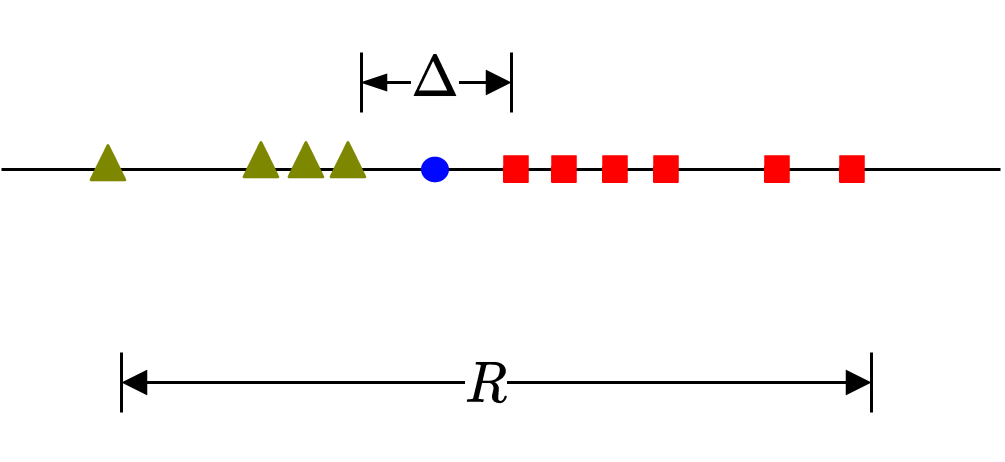
\includegraphics[width=.7\linewidth]{/home/mridul/Desktop/iitd_rishi_laptop/backups/ELL888/margin_func.png}
    \caption{\label{fig:1}Data points $\in\mathbb{R}^1$}
\end{figure}
\begin{figure}[!htbp]
    \centering
    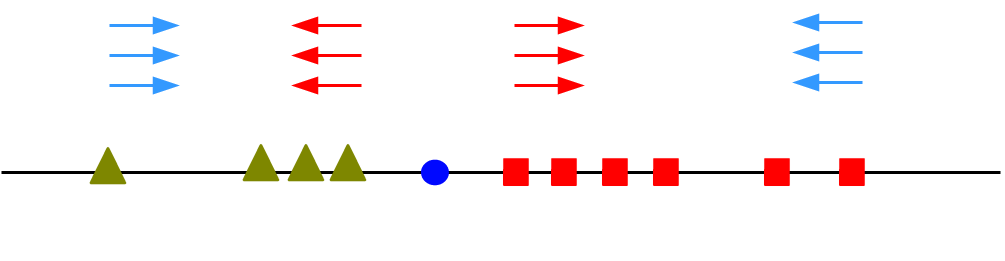
\includegraphics[width=.7\linewidth]{/home/mridul/Desktop/iitd_rishi_laptop/backups/ELL888/margin_func2.png}
    \caption{\label{fig:2}The red arrows are operations on margin and blue
    arrows on radius}
\end{figure}
\subsubsection{MCM formulations}
The mathematical formulations of MCM~\cite{MCM} starts by defining a
mathematical quantity $h_{MCM}$ as
\begin{equation}
    h_{MCM}=\frac{\max_{i=1,2,\dotsc,M}\lVert u^Tx_i+v\rVert}{\min_{i=1,2,\dotsc,M}\lVert u^Tx_i+v\rVert}
\end{equation}
where it is assumed that the separating hyperplane is $u^Tx+v=0$. It is assumed
that the data is linearly separable.\par
Augmenting the data vectors to have a feature whose value is always 1, and
concatenating the weight vector, we have $\hat{x}_i\gets\{x_i;1\}$ and
$\hat{u}\gets \{u;v\}$. Then the hyperplane goes through the origin in the
$\mathbb{R}^{(n+1)}$ space.\par
Then, the margin $\Delta$ is given by
\begin{equation}
    \Delta=\min_{i=1,2,\dotsc,M}\frac{\lVert\hat{u}^T\hat{x}_i\rVert}{\lVert\hat{u}\rVert}
\end{equation}
and the radius is just $R=\max_{i=1,2,\dotsc,M}\lVert\hat{x}_i\rVert$. So, the
ration of interest $\dfrac{R}{\Delta}$ is given by:
\begin{equation}
    \frac{R}{\Delta}=\frac{\max_{i=1,2,\dotsc,M}\lVert\hat{x}_i\rVert}{\min_{i=1,2,\dotsc,M}\frac{\lVert\hat{u}^T\hat{x}_i\rVert}{\lVert\hat{u}\rVert}}=\frac{\max_{i=1,2,\dotsc,M}\lVert\hat{u}\rVert\lVert\hat{x}_i\rVert}{\min_{i=1,2,\dotsc,M}\lVert\hat{u}^T\hat{x}_i\rVert}
\end{equation}
And using the Cauchy-Schwarz inequality ($\lVert a^Tb\rVert\le\lVert
a\rVert\lvert b\rVert$)
\begin{equation}
    \frac{R}{\Delta}\ge\frac{\max_{i=1,2,\dotsc,M}\lVert\hat{u}^T\hat{x}_i\rVert}{\min_{i=1,2,\dotsc,M}\lVert\hat{u}^T\hat{x}_i\rVert}=\frac{\max_{i=1,2,\dotsc,M}\lVert u^Tx_i+v\rVert}{\min_{i=1,2,\dotsc,M}\lVert
    u^Tx_i+v\rVert}
\end{equation}
Thus
\begin{align}
    h_{MCM}&\le\frac{R}{\Delta}\\
    \Rightarrow
    h_{MCM}^2&\le\left(\frac{R}{\Delta}\right)^2<1+\left(\frac{R}{\Delta}\right)^2
\end{align}
From equation~\ref{vcbound} we have for large dimensional data:
\begin{equation}
    h\le 1+\left(\frac{R}{\Delta}\right)^2
\end{equation}
Thus $\exists\beta\in\mathbb{R}^+,$ such that $h\le\beta h_{MCM}^2$. Also since,
$h_{MCM}^2\ge 1$ and VC-dimension satisfies $h\ge 1$,
$\exists\alpha\in\mathbb{R},\alpha>0$ such that $\alpha h_{MCM}^2\le h$.
Combining the two we have $\exists \alpha,\beta > 0, \alpha,\beta\in\mathbb{R}$
such that
\begin{equation}
    \alpha h_{MCM}^2\le h\le\beta h_{MCM}^2
\end{equation}
That is $h^2_{MCM}$ is an exact bound on the VC dimension $h$. And since the
data is linearly separable, $u^Tx_i+v\ge 0$ if $y_i=1$ and $u^Tx_i+v\le 0$ if
$y_i=-1$. Thus $\lVert u^Tx_i+v\rVert$ can be written as $y_i(u^Tx_i+v)$. Thus
the machine capacity can be minimized by keeping $h_{MCM}^2$ as small as
possible.
\begin{equation}
    \underset{u,v}{\operatorname{minimize}}\; h_{MCM}=\frac{\max_{i=1,\dotsc,M}y_i(u^Tx_i+v)}{\min_{i=1,\dotsc,M}y_i(u^Tx_i+v)}
\end{equation}
Further the authors show that the above formulation can be further simplified
by writing:
\begin{align}
    &h_{MCM}=\frac{g}{l}\\
    &\min_{u,v,g,l}\frac{g}{l}\\
    &g\ge y_i(u^Tx_i+v),\quad i=1,\dotsc,M\\
    &l\le y_i(u^Tx_i+v),\quad i=1,\dotsc,M
\end{align}
Using Charnes-Cooper transformation, introducing $p=\frac{1}{l}$
\begin{align}
    &\min_{u,v,g,l,p}g\cdot p\\
    &g\cdot p\ge y_i(p\cdot u^Tx_i+p\cdot v),\quad i=1,\dotsc,M\\
    &l\cdot p\le y_i(p\cdot u^Tx_i+p\cdot v),\quad i=1,\dotsc,M\\
    &p\cdot l=1
\end{align}
Denoting $w\stackrel{\Delta}{=}p\cdot u,b\stackrel{\Delta}{=}p\cdot v$ and
noting that $p\cdot l=1$
\begin{align}
    &\label{eq:1}\min_{w,b,h}h\\
    &\label{eq:2}h\ge y_i(w^Tx_i+b),\quad i=1,\dotsc,M\\
    &\label{eq:3}1\le y_i(w^Tx_i+b),\quad i=1,\dotsc,M
\end{align}
Equations~\ref{eq:1}-\ref{eq:3} define the Minimal Complexity Machine (MCM). And
it is trained by solving the Linear Programming Problem defined above.
\subsubsection{Generalizing the MCM}
The MCM above is further generalized to allow for classification errors by
introducing slack variables.
\begin{align*}
    &\min_{w,b,h,q}h+C\cdot\sum_{i=1}^Mq_i\\
    &h\ge y_i(w^Tx_i+b)+q_i,\quad i=1,\dotsc,M\\
    &1\le y_i(w^Tx_i+b)+q_i,\quad i=1,\dotsc,M\\
    &q_i\ge 0\quad i=1,\dotsc,M
\end{align*}
And for the non-linear case using Kernels
\begin{align}
    &\min_{w,b,h,q}h+C\cdot\sum_{i=1}^Mq_i\\
    &h\ge y_i(w^T\phi(x)_i+b)+q_i,\quad i=1,\dotsc,M\\
    &1\le y_i(w^T\phi(x)_i+b)+q_i,\quad i=1,\dotsc,M\\
    &q_i\ge 0\quad i=1,\dotsc,M
\end{align}
\clearpage


	
	\bibliographystyle{plain}
	\begin{thebibliography}{10}
		\bibitem{mr:random}
	Cormen TH, Leiserson CE, Rivest RL, Stein C. 
		\newblock {\em Introduction to algorithms.}.
		\newblock MIT press.	2009 Jul 31
	\end{thebibliography}
	
	
	
\end{document}
